\chapter{Swaps and Bootstrapping}
\label{sec:swaps-and-bootstrapping}

In this Chapter the Overnight Index Swap contract is reviewed. Besides the financial arguments another very important mathematical technique is 
introduced: the \emph{bootstrapping}.

\section{Overnight Index Swap}
\label{overnight-index-swap}

Interest rate swaps (IRS), that will be described in a later Chapter, are generally used to mitigate the risks of interest rates fluctuations or to benefit from 
expected decreasing rates.
Overnight Index Swaps (OIS) are a particular kind of IRS which pay a floating coupon, determined by overnight rate fixings over the reference periods, against 
a fixed coupon. An OIS in general is defined by:

\begin{itemize}
\tightlist
\item
  a notional amount $N$;
\item
  a starting date $d_0$;
\item
  a sequence of payment dates $d_1,...,d_n$;
\item
  a fixed rate $K$.
\end{itemize}

For simplicity in the following we are assuming that both fixed and floating legs have the same notional and payment dates, although this is not necessarily 
always the case in practice. We will always look at these products from the point of view of the \textbf{receiver of the floating leg}.

\subsection{OIS Valuation}\label{ois-valuation}
The net present value (NPV) of such products is defined as the sum of the discounted cash-flows of each leg.

\subsubsection{Floating leg}\label{floating-leg}
At each payment date, the floating leg pays a cash-flow determined as follows:

\begin{equation}
f_{\mathrm{float},~i} = N \Bigg\{\prod_{d=d_{i-1}}^{d=d_i-1}\Big(1+r_{\mathrm{O/N}}(d)\cdot\frac{1}{360}\Big) -1 \Bigg\}
\label{eq:floating_ois}
\end{equation}

Strictly speaking this formula is valid for an \euro STR swaps (i.e. for OIS swaps in EUR) other currencies might have different conventions. 
The $\frac{1}{360}$ fraction appears because \euro STR rates are quoted using the ACT/360 day-count convention. 

In addition we are making the simplifying assumption of ignoring weekends and holidays, so we assume that each overnight rate is valid for only one day. 
The sum of the discounted expected values of these cash-flows is

\begin{equation}
\mathrm{NPV}_{\mathrm{float}} = \sum_{i=1}^{n}D(d_i)\mathbb{E}[f_{\mathrm{float},~i}]
\end{equation}
where $D(d)$ is the discount factor with expiry $d$. Eq.~\ref{eq:floating_ois} can be simplified by using the same no-arbitrage argument exploited in 
Section~\ref{calculating-forward-rates}. Expanding the product indeed

\begin{equation*}
\prod_{i=d}^{d'} (1+r_i\tau_1) = \underbrace{(1+r_{d,d+1}\tau_1)\underbrace{(1+r_{d+1,d+2}\tau_1)\ldots\underbrace{(1+r_{d'-2,d'-1}\tau_1)(1+r_{d'-1,d'}\tau_1)}_{\textstyle =(1+r_{d'-2,d'}\tau_{d'-2,d')}}}_{\textstyle =(1+r_{d+1,d'}\tau_{d+1, d'})}}_{\textstyle =(1+r_{d,d'}\tau_{d,d'})}
\end{equation*}
\noindent
Using Eq.~\ref{eq:no_arbitrage_r} the resulting expression can be written in terms of spot rates
\begin{equation*}
(1+r_{d,d'}\tau_{d,d'}) = \left(\cfrac{1+r_{0, d'}\tau_{0,d'}}{1+r_{0,d}\tau_{0,d}}\right)
\end{equation*}
\noindent Finally it is useful to express the expectation in terms of discount factors

\begin{equation*}
\mathbb{E}[f_{\mathrm{float},~i}] = N\cdot\Big(\cfrac{D_{\mathrm{OIS}}(0, d_{i-1})}{D_{\mathrm{OIS}}(0, d_{i})} - 1\Big)\qquad \mathrm{where}\ D_{\mathrm{OIS}}(0,d)=\cfrac{1}{1+r_{0,d}\tau_{0,d}}
\end{equation*}

\begin{equation*}
\mathrm{NPV}_{\mathrm{float}} = N\cdot \sum_{i=1}^{n}D(d_i) \Big(\cfrac{D_{\mathrm{OIS}}(d_{i-1})}{D_{\mathrm{OIS}}(d_{i})} - 1\Big)
\end{equation*}
From what has been said in Section~\ref{sec:financial-crisis} we have that $D = D_{\mathrm{OIS}}$ and the NPV simplifies to

\begin{equation}
	\begin{split}
		\mathrm{NPV}_{\mathrm{float}} & = N\cdot\sum_{i=1}^{n}[D(d_{i-1}) - D(d_i)] =  \\
		&= N\cdot[(D(d_{0}) - D(d_{1})) + (D(d_{1}) - D(d_{2})) + ... + (D(d_{n-1}) - D(d_{n}))]\\
		&= N \cdot [D(d_0) - D(d_n)]
	\end{split}
\end{equation}

%The correct curve to use for discounting the flows of a collateralized contract, like OIS, is the one associated with the collateral. Since OIS contracts are collateralized with cash, and cash accrues daily interest at the overnight rate, the OIS curve is itself the correct curve with which to discount the flows of an OIS contract ! 
%From what has been said in Section~\ref{sec:financial-crisis}
%Since the financial crisis, in the Euro area the rates used for
%discounting has been the EONIA rates. Similarly, in other jurisdictions
%it has been used other overnight rates such us Fed fund rates in USA.
%This practice is consistent with the daily remuneration of the
%collateral (i.e. cash given or received as mitigants for credit risk
%arising from the mark to market of the derivatives contract).
%For arbitrage consideration the discounting curve of future cash flows
%in a derivative contract can only be the one derived from the rates
%applied for the collateral.
%
%So we have that \(D = D_{\mathrm{OIS}}\) and the NPV simplifies to

\subsubsection{Fixed leg}\label{fixed-leg}

The calculation for the fixed leg is simpler; each cash flow is equal to

\begin{equation}
f_{\mathrm{fixed},~i}=N\cdot K\cdot \frac{d_i - d_{i-1}}{360}
\end{equation}
so the NPV of the fixed leg is

\begin{equation}
\mathrm{NPV}_{\mathrm{fixed}} = N\cdot K\cdot \sum_{i=1}^{n}D(d_{i})\frac{d_i - d_{i-1}}{360}
\end{equation}

%\subsection{\texttt{OvernightIndexSwap} %Class}\label{discount-factor-determination-from-market-quotes}

\begin{finmarkets}
Our ultimate goal is to take a series of Overnight Index Swap quotations, and determine the discount factors implied by their prices. To do this we 
implement a class to describe an OIS and compute its value given a particular discount curve. Then we will use this class with a numerical optimizer 
to \emph{invert} the relationship between NPV and discount curve so that the \emph{implied} discount factors can be determined from OIS market quotes.
The attributes of the \texttt{OvernightIndexSwap} class are the necessary parameters to fully describe an Overnight Index Swap, i.e. the nominal of the 
contract, its start date and maturity and the rate of the fixed leg. The class has methods to calculate the net present value and the fair value strike 
which computes the rate which would make the OIS NPV zero. The implementation of the former relies on the formulas derived above, while the latter is 
based on the simple observation that if the NPV is 0 the expressions for the NPV of each swap leg must equal, then just solve for $K$:

\begin{equation}
\begin{gathered}
K \sum_{i=1}^{n}D(d_{i})\cfrac{d_i - d_{i-1}}{360} = [D(d_0) - D(d_n)] \\
K = \cfrac{[D(d_0) - D(d_n)]}{\sum_{i=1}^{n}D(d_{i})\cfrac{d_i - d_{i-1}}{360}}
\end{gathered}
\end{equation}
\end{finmarkets}

\pythoncodenon{code/bootstrap_ois.py}

Let's test the class using the following discount curve: 
\href{https://github.com/matteosan1/finance_course/raw/master/input_files/discount_factors_2022-10-05.xlsx}{discount\_factors\_2022-10-05.xlsx}.

\pythoncodenon{code/bootstrap_3.py}

\begin{ioutput}
-2,162.61 EUR
\end{ioutput}

\section{Constructing the Yield Curve with Bootstrap}
\label{sec:the-bootstrapping-technique}

In finance, the \emph{bootstrap algorithm} is a method for constructing a yield curve (and other curves) from prices of coupon-bearing products, e.g. bonds and swaps. 
The term structure of spot rates is obtained from the product yields by solving for them recursively, by \emph{forward substitution}. 
The beauty of bootstrap resides on that using only a few carefully selected products, it is possible to derive forward and spot rates for all maturities.

This algorithm relies on the assumption that market quotes represent the \textbf{fair price} of the contracts such that their NPVs are null. The fair price 
is an estimate of what a willing buyer would pay a willing seller for a given asset, assuming both have a reasonable knowledge of the asset's worth.

To illustrate bootstrapping let's consider some bonds (yearly coupon of 4\%, 5\%, 6\%, 7\% and 8\% respectively) with maturities ranging from 1 to 5 years, 
each having a value of 100 and traded at par. 

To determine the yield curve proceed as follows:
\begin{enumerate}
\item at the end of the first year the $1^{st}$ bond will pay a coupon of 4 (= 100 * 4\%) plus the principal (=100) which sums up to 104 while the bond is 
trading at 100. The implied 1-year spot rate $S_{1y}$ can be calculated from $\mbox{100} = \mbox{104} / (1 + S_{1y})$;
\item at the end of second year the sum of the cash flows of the $2^{nd}$ bond can be compared to its trading price to compute the 2-year spot rate $S_{2y}$ 
from $\mbox{100} = \mbox{5} / (1 + S_{1y}) + \mbox{105} / (1 + S_{2y})^{2}$ where the previously derived value of $S_{1y}$ is used;
\item similarly at the end of third year we get the 3-year spot rate 
$S_{3y}$ as $\mbox{100} = \mbox{6} / (1 + S_{1y}) + \mbox{6} / (1 + S_{2y})^{2} + \mbox{106} / (1 + S_{3y})^{3}$, using $S_{1y}$ and $S_{2y}$ computed before;
\item and so on for all the remaining bonds\ldots
\end{enumerate}

Putting all together we can construct a system of equations

\begin{equation}
\begin{cases}
100 = \cfrac{104}{(1 + S_{1y})} \\
100 = \cfrac{5}{(1 + S_{1y})} + \cfrac{105}{(1 + S_{2y})^{2}} \\
100 = \cfrac{6} {(1 + S_{1y})} + \cfrac{6}{(1 + S_{2y})^{2}} + \cfrac{106} {(1 + S_{3y})^{3}} \\
100 = \cfrac{7} {(1 + S_{1y})} + \cfrac{7} {(1 + S_{2y})^{2}} + \cfrac{7} {(1 + S_{3y})^{3}} + \cfrac{107} {(1 + S_{4y})^{4}} \\
100 = \cfrac{8} {(1 + S_{1y})} + \cfrac{8} {(1 + S_{2y})^{2}}+ \cfrac{8} {(1 + S_{3y})^{3}} + \cfrac{8} {(1 + S_{4y})^{4}} + \cfrac{108} {(1 + S_{5y})^{5}}
\end{cases}
\label{eq:fifth_year_rate}
\end{equation}

This system can be solved quite easily: $S_{1y}$ can be derived from the first equation, $S_{2y}$ from the second, $S_{3y}$ from the third\ldots So

\begin{equation}
100 = 104 / (1 + S_{1y})\quad\Rightarrow\quad S_{1y} = 104/100 - 1 = 4\%
\end{equation}
Moving to the second equation:
\begin{equation}
\begin{split}
& 100 = 5 / (1 + 0.04) + 105 / (1 + S_{2y})^{2}\quad\Rightarrow\quad S_{2y}^2  + 2 S_{2y}  - 0.103030 = 0 \\
& S_{2y} = - 1 \pm \sqrt{1 + 0.103030} = \begin{cases}\text{\sout{-2.05023}} \\ 0.0502\end{cases}
\end{split}
\end{equation}
where the first solution has been discarded because negative. This equation can also be solved in \texttt{python} with \texttt{numpy.roots}.

From the third equation on, it is not as simple to solve them analytically since they involve third order (or more) equations, but is still possible to 
compute a numerical solution.
As an example assume all rates up to the fourth year have been calculated and just the last one needs to be determined. The last column of Table~\ref{tab:rates} 
provides the terms to fill the yield curve.

\begin{table}[htb]
\begin{center}
\begin{tabular}{|c|c|c|c|}
\hline
\textbf{years} & \textbf{coupon rate} & \textbf{bond price} & \textbf{spot rate} \\
\hline
1 & 1.00 \% & 100 & 4.00\% \\
\hline
2 & 2.00 \% & 100 & 5.02\% \\
\hline
3 & 3.00 \% & 100 & 6.08\% \\
\hline
4 & 4.00 \% & 100 & 7.19\% \\
\hline
5 & 5.00 \% & 100 & ??? \\
\hline
\end{tabular}
\end{center}
\caption{Table reporting maturity, coupon, bond price and implied spot rate for the example outlined in the text.}
\label{tab:rates}
\end{table}

To solve the last of Eq.~\ref{eq:fifth_year_rate} numerically one of the root finding algorithm illustrated in Section~\ref{sec:root_finding} can be used. 
In this case \texttt{scipy.optimize.brentq} is used, it finds zeros of a user-defined function within a validity interval.

In Figure~\ref{fig:fifth_year_rate} the equation is plotted as a function of $S_{5y}$. It already gives us an idea of the expected result, the rate value 
which solves the equation should be around 0.08.

\begin{figure}[htb]
  \centering
  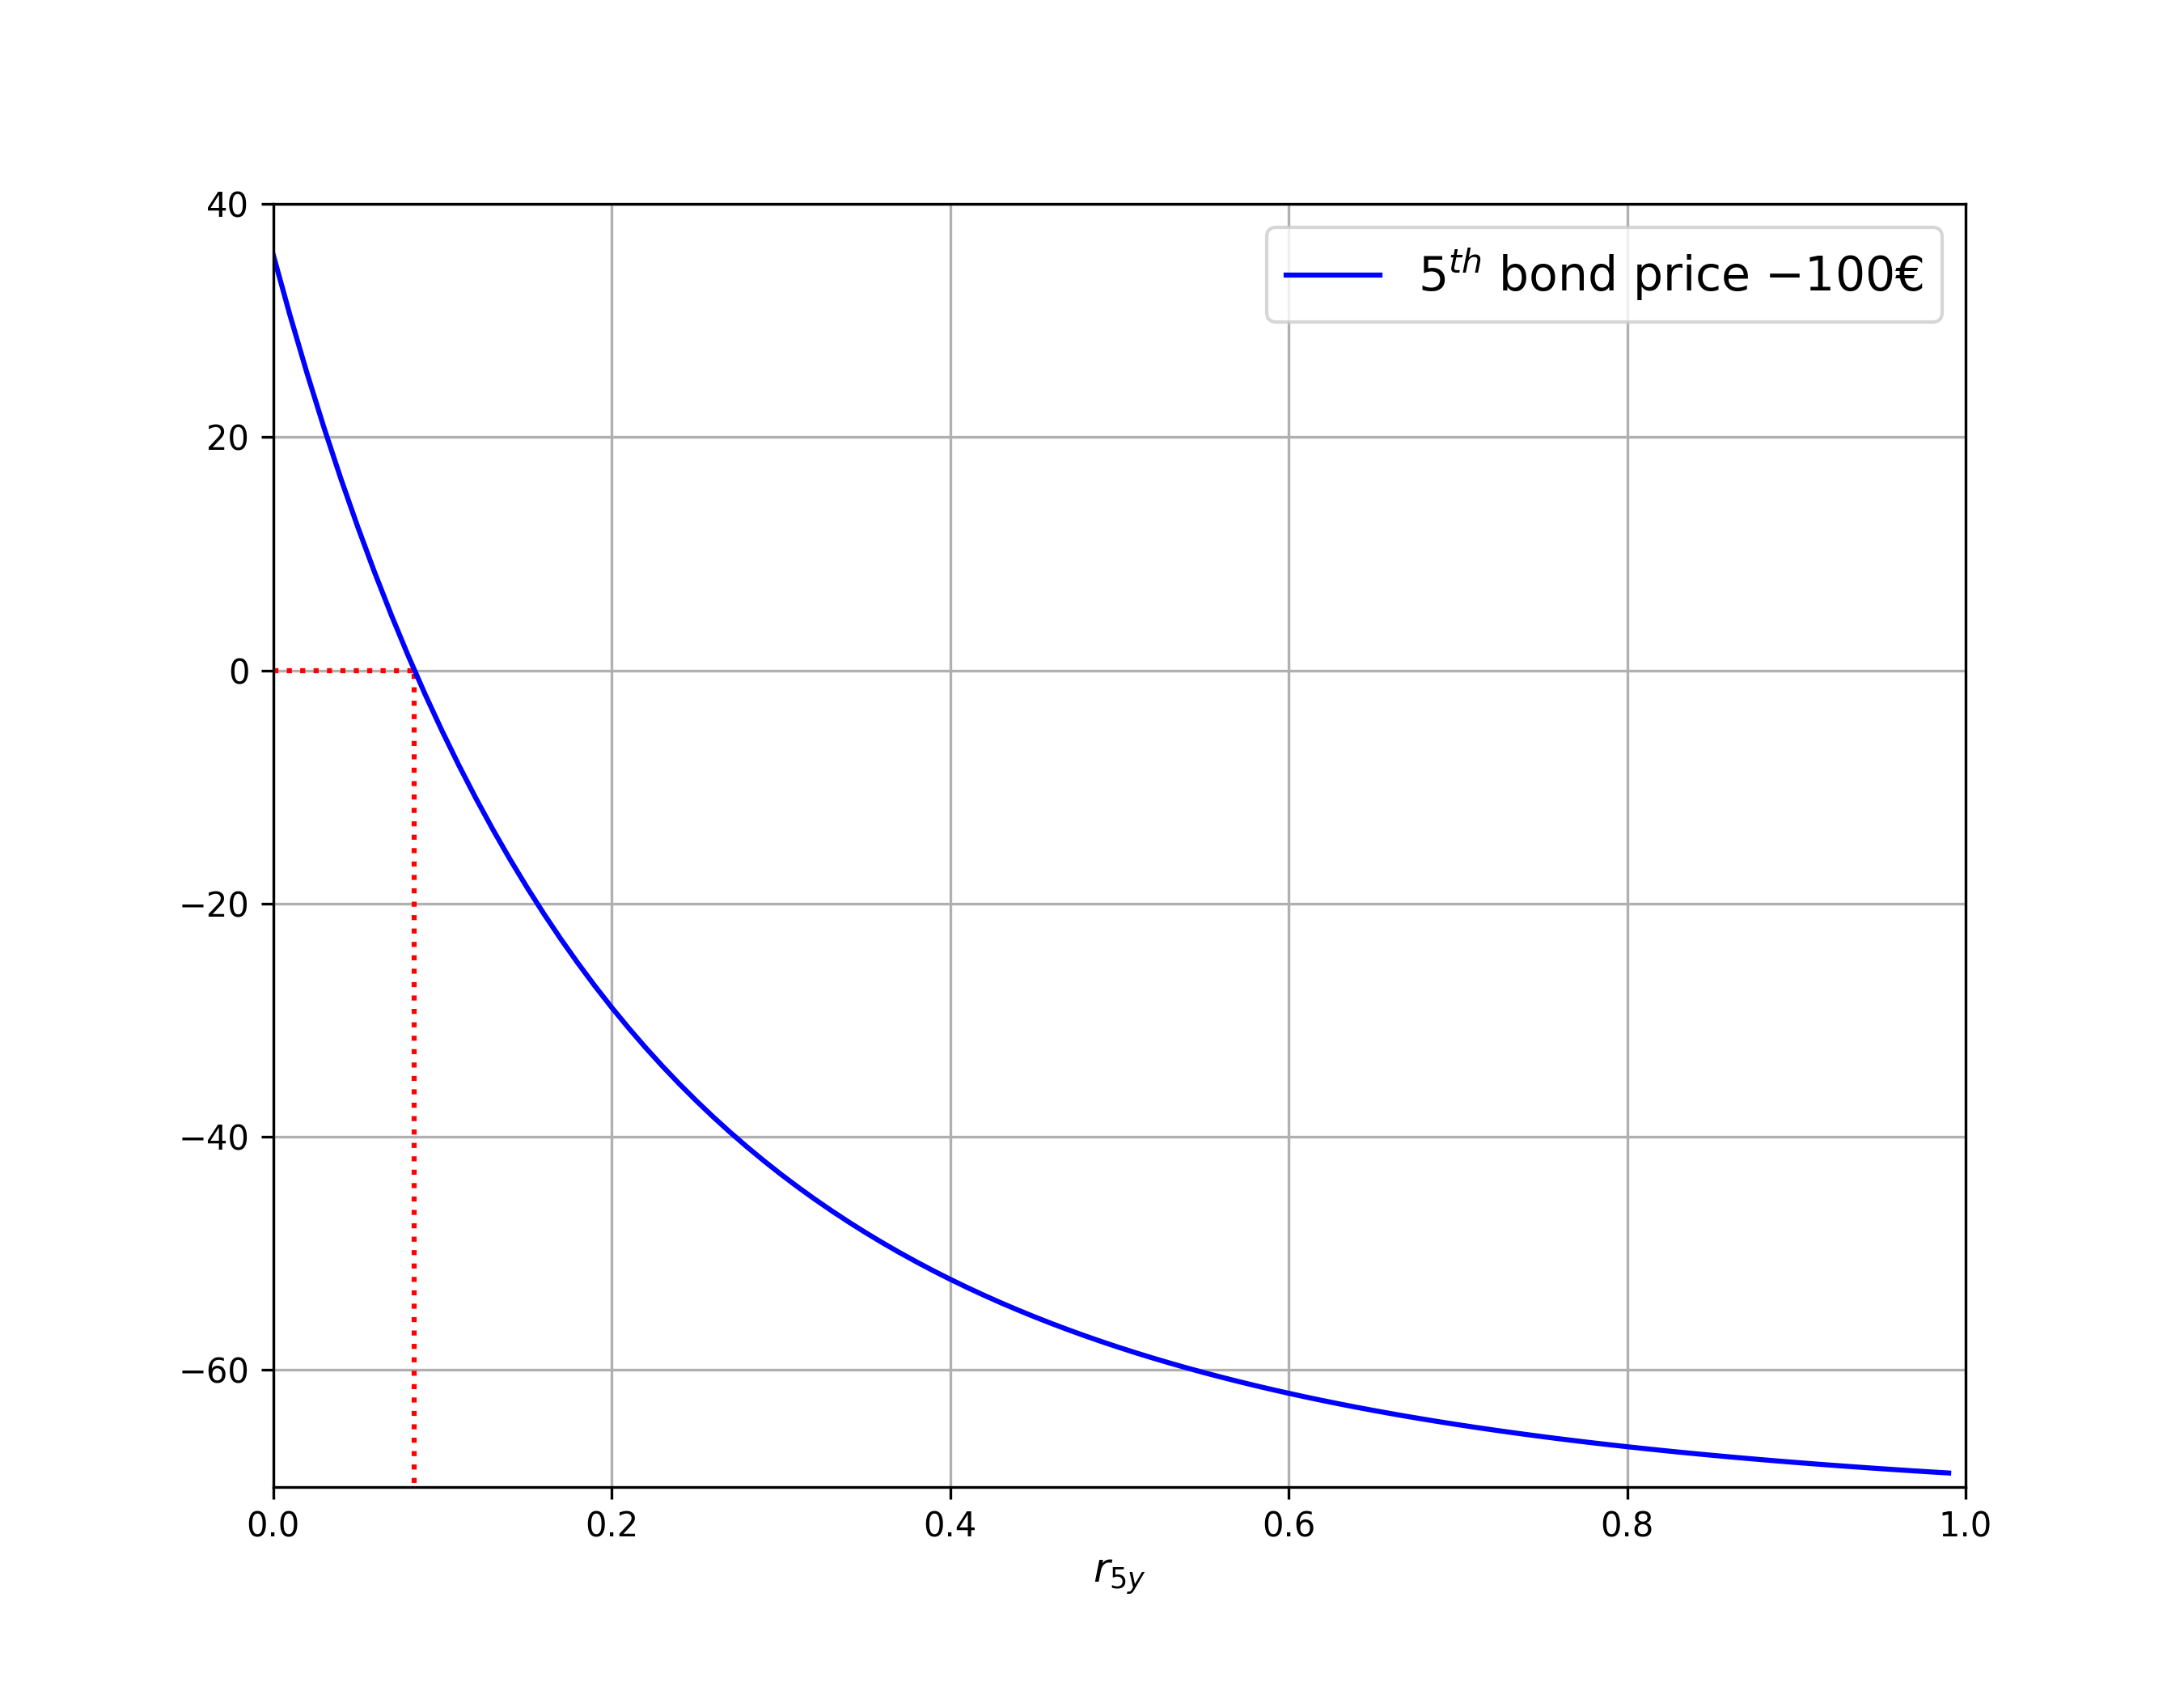
\includegraphics[width=0.7\textwidth]{figures/bond_5_plot.png}
  \caption{Plot of the discounted cash flow of bond 5 as a function of the 5 year spot rate.}
  \label{fig:fifth_year_rate}
\end{figure}

\pythoncodenon{code/bootstrap_4.py}

\begin{ioutput}
5y rate: 0.0836
\end{ioutput}

The very same mechanism can be generalized and extended to other maturities to get a more detailed yield curve. In general terms the previous system becomes

\begin{equation}
\begin{cases}
f_1(S_1, p_1) = 0 \\
f_2(S_1, S_2, p_2) = 0 \\
f_3(S_1, S_2, S_3, p_3) = 0 \\
f_4(S_1, S_2, S_3, S_4, p_4) = 0 \\
\cdots
\end{cases}
\end{equation}
where $S_i$ are the unknown spot rates and $p_i$ the market quotes of the considered products. The iterative procedure we have applied before exploits the first equation to find $S_1 = f_1^{-1}(p_1)$, the second to find $S_2 = f_2^{-1}(S_1, p_2)$ and so on. Each equation determines exactly one spot rate which is not already determined by the others.

\subsection{Bootstrapping of Discount Curve}

From what we have seen the discount curve can be \emph{bootstrapped} by successively calibrating it to return the input product market quotes.
Let's implement the outlined procedure in \texttt{python}, the first step is to choose the set of contracts to use in the minimization.

Our choice concerns a set of Overnight Index Swaps indexed on \euro STR, in Fig.~\ref{fig:icap} the used quotes.
 
\begin{figure}[bth]
	\centering
	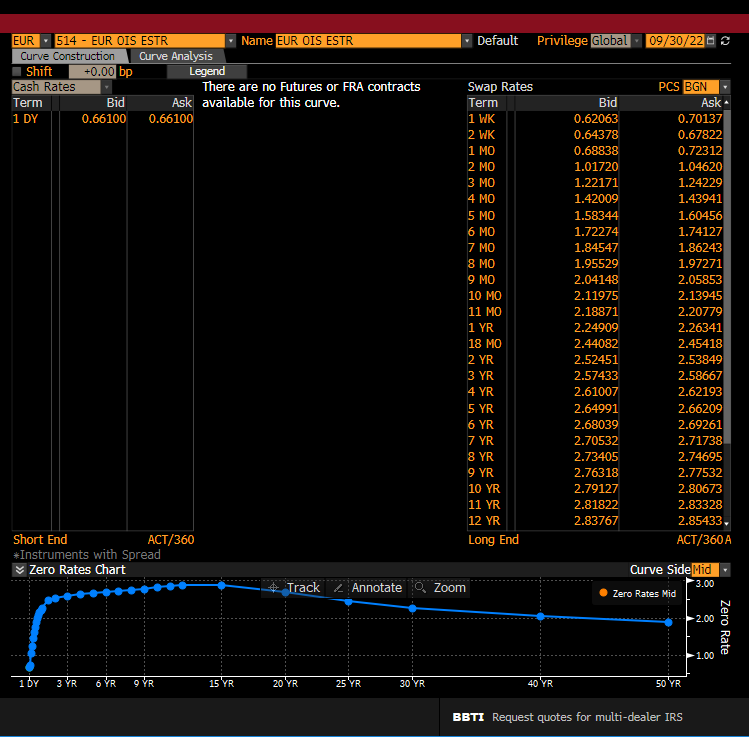
\includegraphics[width=1.\linewidth]{figures/bbg_ois}
	\caption{Screenshot of OIS market quotes from Bloomberg as of 2022-09-30.}
	\label{fig:icap}
\end{figure}

Note that interest rate swap quotes vary from standard prices of commonly traded instruments, they can be puzzling but are effectively interest rates 
(i.e. the rate of the fixed leg).

The resulting dateset is stored in (\href{https://github.com/matteosan1/finance_course/raw/master/input_files/ois_2024_10_14.xlsx}{\texttt{ois\_2024\_10\_14.xlsx}}).

\pythoncodenon{code/bootstrap_6.1.py}

\begin{ioutput}
  maturities    quotes     
  7D          3.414000
  14D         3.295500
  1M          3.229000
  2M          3.209205
  3M          3.127103  
\end{ioutput}

Now using a very simple \texttt{Bootstrap} class we are going to construct the discount curve by adding at each iteration a new pillar given by the 
maturity of the corresponding OIS. 

So the 7D swap depends on the discount factor seven days in advance from today. 
At the beginning of the Chapter we said that the OIS market quotes represent their \emph{fair} prices (i.e. the price which buyer and seller happily agree for 
the contract). The bootstrap will set it by requiring the OIS net present value to be zero (this is the objective function), task that can be easily performed
using one the root finding algorithms outlined in~\ref{sec:root_finding}. 

Moving to the 14D OIS, its NPV depends on the 7D (already found) and 14D discount factors, so the second parameter will be 
determined by again requiring the net present value to be 0. The process iteratively will find a new discount factor for each OIS in the list defining the entire
discount curve.

\pythoncodenon{code/bootstrap_6.2.py}

Finally we have created the discount curve implied by the market quotes of our swaps (see Fig.~\ref{fig:discount_curve}), so we can compute some implied 
rates.

\pythoncodenon{code/bootstrap_6.3.py}

\begin{ioutput}
40y df: 0.622
40y rate: 0.0028
\end{ioutput}

\begin{figure}[htb]
	\centering
	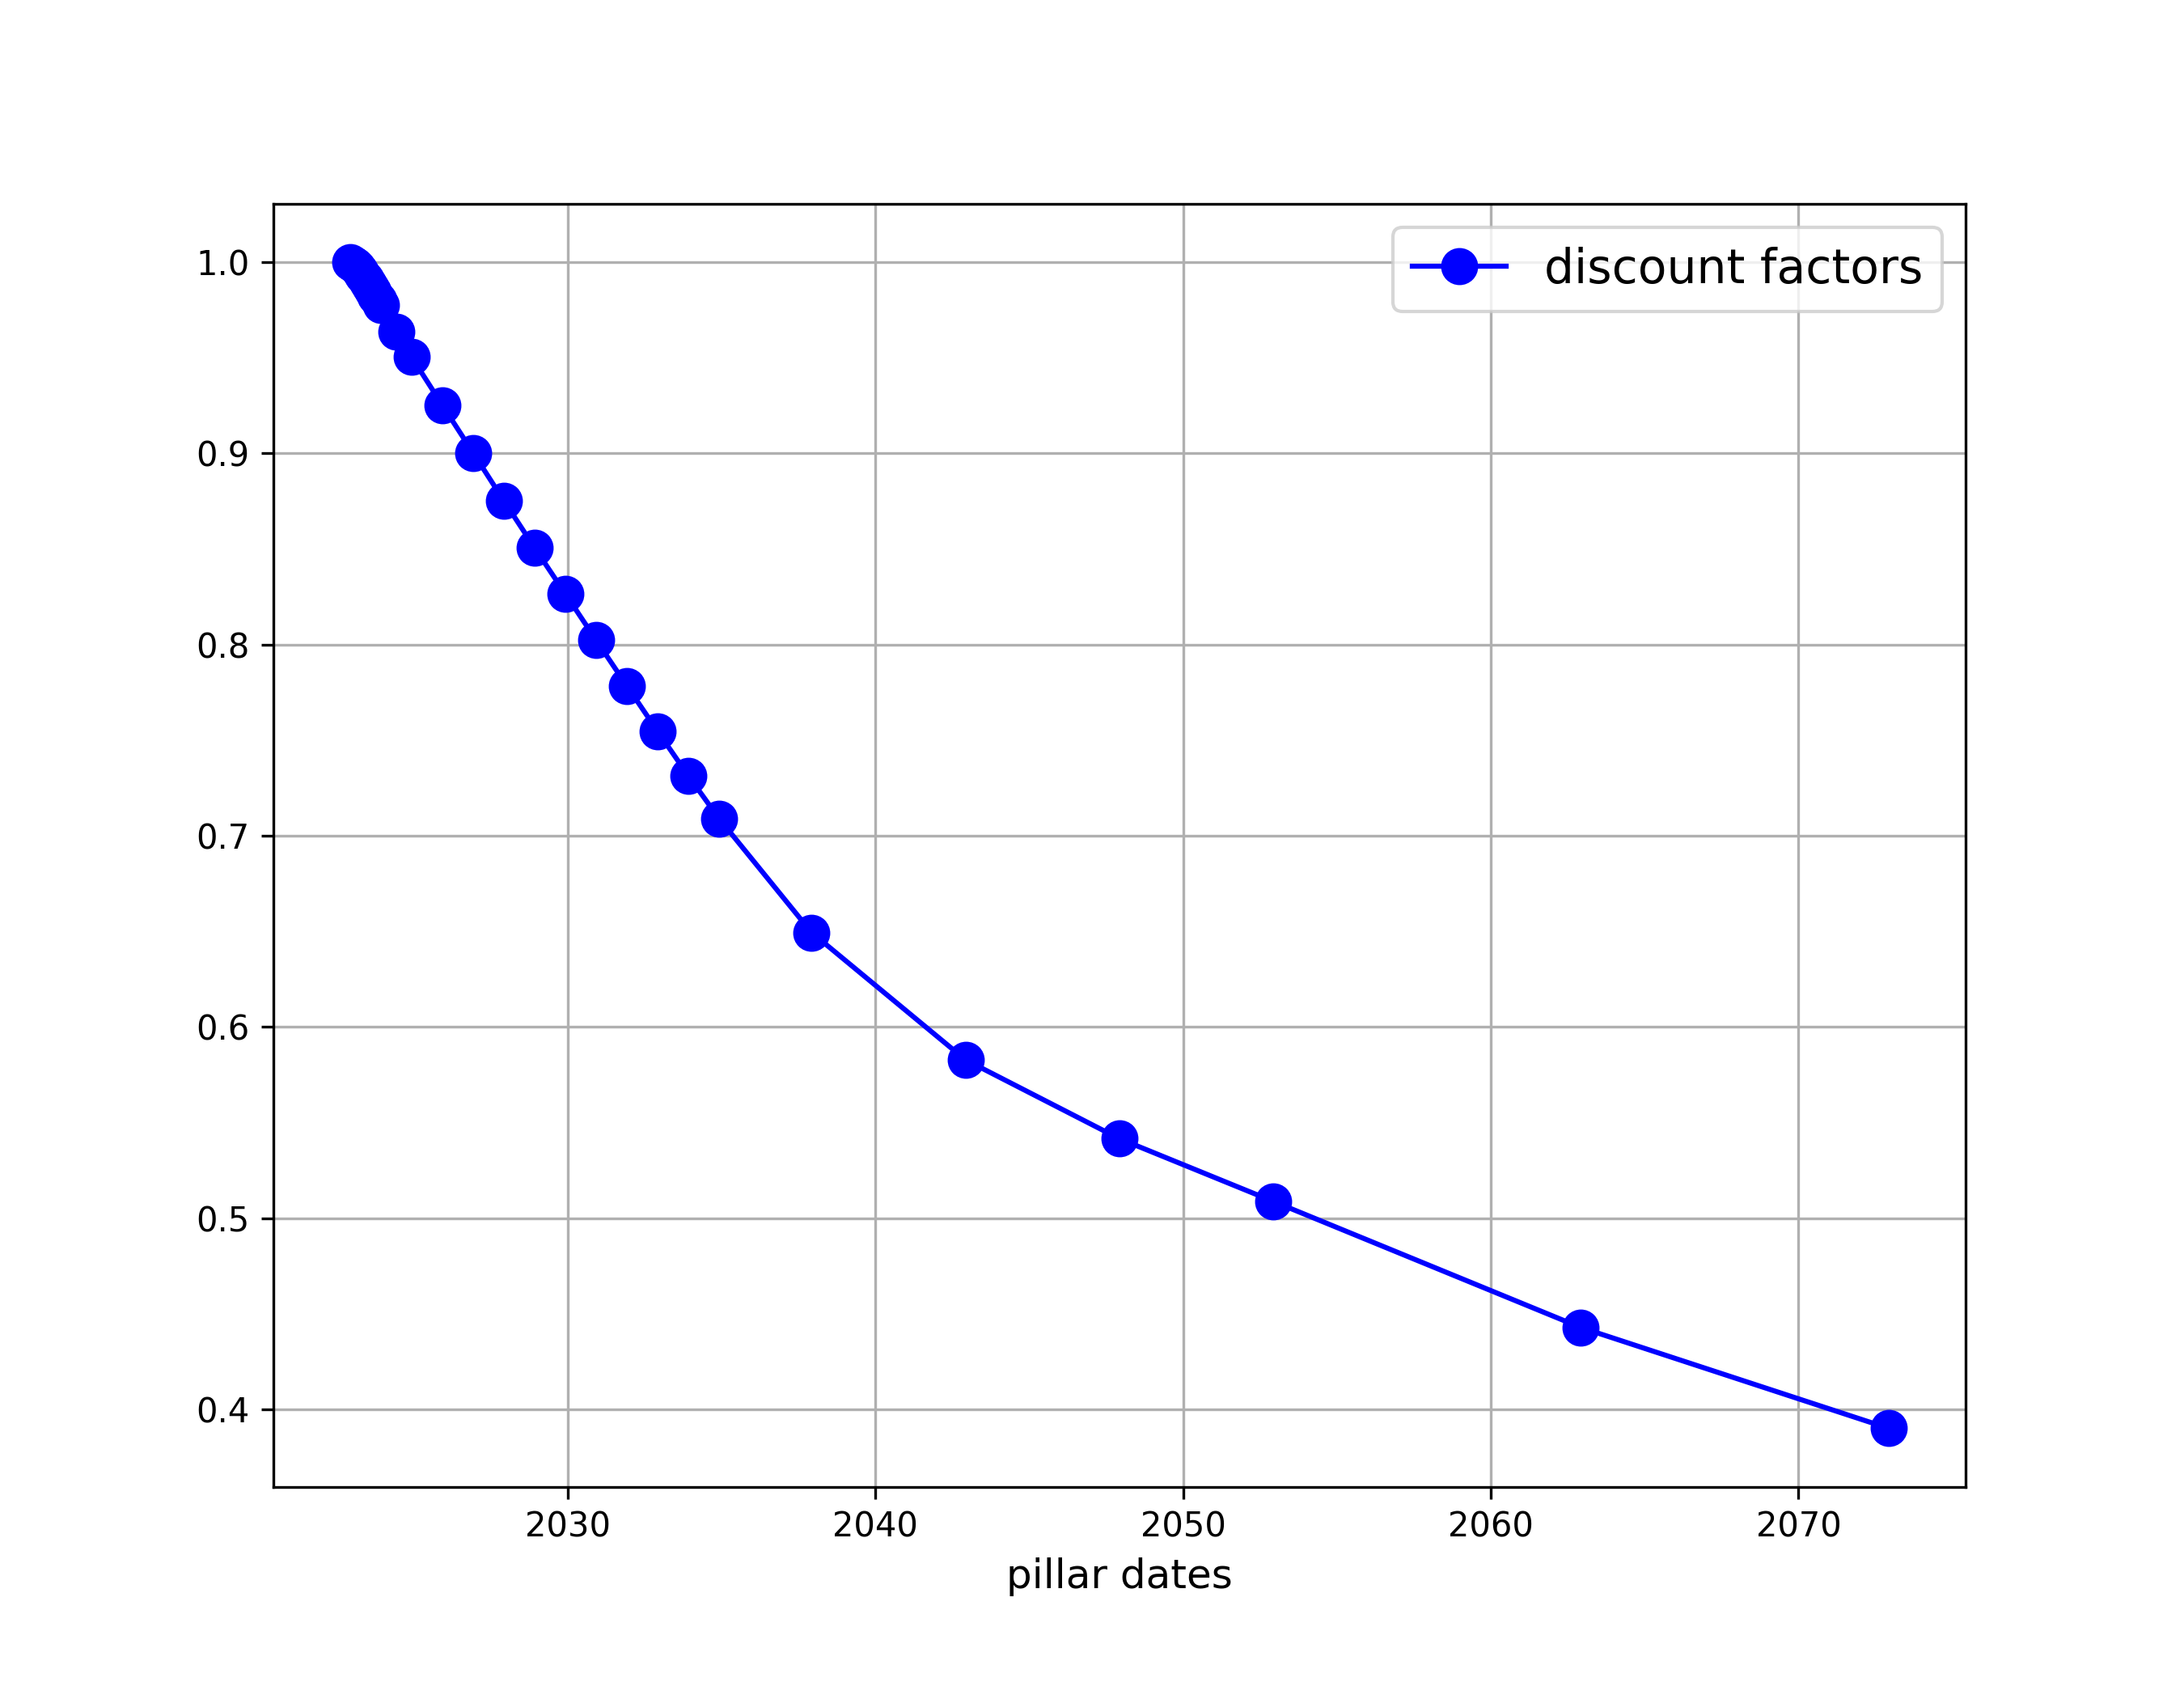
\includegraphics[width=0.7\textwidth]{figures/example_discount_curve}
	\caption{Plot of the discount curve implied by Overnight Index Swap market quotes.}
	\label{fig:discount_curve}
\end{figure}

\subsection{Bootstrapping as Minimization Problem}
\label{sec:bootstrap_as_minimization}

The bootstrap algorithm can alternatively be seen under another point of view. Define a vector of spot rates $\mathbf{S} = (S_1, S_2, S_3, \ldots)$ and 
seek for a particular set $\mathbf{\hat{S}}$ which solves the following equation:

\begin{equation}
F = f_1^2(\hat{S}_1,p_1) + f_2^2(\hat{S}_1, \hat{S}_2,p_2) + f_3^2(\hat{S}_1, \hat{S}_2, \hat{S}_3,p_3) + f_4^2(\hat{S}_1, \hat{S}_2, \hat{S}_3, \hat{S}_4,p_4) + \ldots = 0
\label{eq:bootstrap_as_minimization}
\end{equation}

Solving Eq.~\ref{eq:bootstrap_as_minimization} is equivalent to find the solution of the system~\ref{eq:fifth_year_rate}.
Under this terms the bootstrap method becomes a \emph{minimization problem}. In fact we need to find $\mathbf{\hat{S}}$ which \emph{minimize} $F$, 
(i.e. makes it as close as possible to 0).

This means that the OIS NPV's should be close to 0 hence the objective function~\ref{eq:bootstrap_as_minimization} becomes

\begin{equation}
\mathrm{Objective Function} = \sum_{i=1}^{n}\mathrm{NPV}^\mathrm{OIS}_i(\mathcal{C})^2
\end{equation}.

Once the OIS characteristics (e.g. nominal, maturity\ldots) have been specified the only unknown parameter in the NPV calculation is the discount 
curve $\mathcal{C}$ (i.e. the minimization algorithm will adjust $\mathcal{C}$ to reach the minimum).

In previous examples the number of minimization parameters, \emph{the degrees of freedom} of the problem, were clear:
\begin{itemize}
\item 1 for the can example, the can radius;
\item 2 for the fence problem, width and height of the field.
\end{itemize}

A discount curve is characterized by a set of pillar dates ($\mathbf{d}$) and a set of discount factors ($\mathbf{x}$), but it hasn't yet been 
identified any constraint on how many points the curve has to be made of (too many or too few points may prevent us from finding the solution).

In practice \textbf{it makes sense to choose the degrees of freedom to match the number of market quotes}. In particular it is wise to choose the pillar 
dates of the discount curve equal to the swap expiry dates, leaving as unknown parameters just the discount factors.

The final version of the optimization problem becomes

\begin{equation}
 \mathrm{min}_{\mathbf{x}} \left\{\sum_{i=1}^{N}\mathrm{NPV}^\mathrm{OIS}_i( \mathcal{C}(\mathbf{x}))^2\right\}
\end{equation}
i.e. finding the minimum of the above expression as a function of the discount factors $\mathbf{x}$.

Notice how each $f_i$ is squared since we want all of them to be minimized at the same time and not only $F$ globally 
(i.e. without the square there may be cancellation effects between the terms of the sum, which makes $F$ zero but not all $f_i$ individually).

Let's repeat the bootstrapping with the swaps defined above. 
#(today's discount factor is fixed to 1 so it is not included among the minimization parameters). 
Note that the objective function has constant additional parameters so they will be passed using \texttt{args} (see Section~\ref{sec:kwargs_args}). 

Set the initial value of the discount factors $x_i^0$ to 1 with a range of variability $[0.01, 10]$. Discount factor 0 will be set fixed to 1.
Finally launch the minimizer to find the discount factors $\mathbf{x}$

\pythoncodenon{code/bootstrap_7.py}

\begin{ioutput}
  message: CONVERGENCE: NORM_OF_PROJECTED_GRADIENT_<=_PGTOL
  success: True
   status: 0
      fun: 1.547769660487322e-12
        x: [ 9.994e-01  9.983e-01 ...  4.428e-01  3.901e-01]
      nit: 7
      jac: [ 2.598e-07  4.056e-07 ...  1.766e-07  4.188e-07]
     nfev: 279
     njev: 9
 hess_inv: <30x30 LbfgsInvHessProduct with dtype=float64>
 \end{ioutput}

A useful cross-check to perform to understand if everything went fine, is the comparison of the objective function value at the beginning and at the end of 
minimization.

\begin{ipythonnon}
print ("Initial objective function value ", objective_function(x0, obs_date, 
                                          pillar_dates, swaps))
print ("Final objective function value ", objective_function(result.x, obs_date,
                                          pillar_dates, swaps))
\end{ipythonnon}
\begin{ioutput}
Initial objective function value  51601443377.52911
Final objective function value  6.013612670431716e-06
\end{ioutput}
The objective function at the end of the minimization is not exactly 0 (and rarely it will be) but its value is small enough for us to be satisfied: 
the initial value was around $10^{10}$ and now it is $10^{-6}$ so several orders of magnitude smaller. This means that with the derived discount curve 
the NPV's of our OIS won't be identically 0 but so small that can be regarded as they would.

\subsection{Discount Factors with Pseudo-inverse}
An alternative procedure to derive discount factors involves matrix inversion and in some special cases the usage of the \emph{pseudoinverse} described in Section~\ref{sec:the-moore-penrose-pseudoinverse}. Details on this algorithm can be found in~\cite{bib:boostrap_pseudoinv}.

Consider a set of $n$ financial instruments (e.g. bonds, futures, swaps, \ldots). The price of such instruments is connected to the discount factors by the following relationship

\begin{equation}
P_i = \sum_{j=0}^{m} C_{i,j} d_j
\label{eq:discounted_cashflows}
\end{equation}
where $P_i$ is the market quote of the $i^{th}$ product, $C_{i,j}$ is the $j^{th}$ cash-flow of the $i^{th}$ product and $d_j$ is the discount factor relative to period $(t_0, t_j)$.
Eq.~\ref{eq:discounted_cashflows} can be written in matrix form

\begin{equation}
\boldsymbol{P} = [C]\boldsymbol{d}
\label{eq:discount_matrix}
\end{equation}
and now $P$ and $d$ are column vectors while $[C]$ is a $n \times m$ matrix where each row element is a cash-flow associated to the row product.

Recalling Section~\ref{solving-systems-of-equations-using-matrix-inverses}, Eq.~\ref{eq:discount_matrix} represents a system of equations which can be solved to determine the unknown $\boldsymbol{d}$.
The sought solution is 
\begin{equation}
\boldsymbol{d} = [C^{-1}] \boldsymbol{P}
\end{equation} 
If matrix $[C]$ is not invertible (i.e. the system of equations is under-determined) $[C^{-1}]$ can be replaced by the optimal approximation $[C^+]$ (i.e. the pseudo-inverse). 

To illustrate the algorithm let's consider again the previous example with five coupon bearing bonds (coupon of 4\%, 5\%, 6\%, 7\% and 8\% respectively) with maturities ranging from 1 to 5 years, each having a value of \euro{100} and traded at par. In this case we have
\begin{equation*}
\boldsymbol{P} = 
\begin{bmatrix}
100 \\
100 \\
100 \\
100 \\
100 
\end{bmatrix}; \quad
[C] = 
\begin{bmatrix}
104 & 0 & 0 & 0 & 0 \\
5 & 105 & 0 & 0 & 0 \\
6 & 6 & 106 & 0 & 0 \\
7 & 7 & 7 & 107 & 0 \\
8 & 8 & 8 & 8 & 108
\end{bmatrix}; \quad \boldsymbol{d} =
\begin{bmatrix}
d_1 \\
d_2 \\
d_3 \\
d_4 \\
d_5 
\end{bmatrix}
\end{equation*}
The \texttt{python} implementation to determine the solution is given in the snippet below. The code use by default the pseudo-inverse since if $[C]$ is invertible holds $[C^+] = [C^{-1}]$. 

\pythoncodenon{code/bootstrap_9.py}

\begin{ioutput}
[0.96153846 0.90659341 0.83765291 0.75756548 0.66938146]	
\end{ioutput}
To determine the corresponding yields just use \texttt{brentq} to solve $d=1/(1+y_n)^{n}$

\begin{ioutput}
yield y1: 0.0400
yield y2: 0.0503
yield y3: 0.0608
yield y4: 0.0719
yield y5: 0.0836
\end{ioutput}
which matches those in Table~\ref{tab:rates}.

In this simple example just bonds were considered but clearly the method can be extended also to other instruments when creating the cash-flow matrix $[C]$.

\section*{Exercises}
%\begin{question}
Consider two 5\% coupon paying bonds (par value of \euro{100}) with the clean market prices of \euro{99.50} and \euro{98.30} and having maturities of 6 months and 1 year respectively.
Determine the spot rate for the 6-month and 1-year bond.  
\end{question}

\begin{solution}
At the end of 6 months the first bond will pay a coupon of \euro{2.5} (= \euro{100} * 5\%/ 2) plus the principal amount (= €100) which sums up to 102.50. To
determine the 6M spot rate we can write the following equation, :

\[ \cfrac{102.5}{(1 + S_{6M}/2)} = 99.5\qquad\Rightarrow\qquad S_{6M} = 2 \cdot \Big( \cfrac{102.5}{99.5} - 1 \Big) =  6.03 \%\]

At the end of another 6 months the second bond will pay a coupon of €2.5
(= €100 * 5\% / 2) plus the principal amount (= €100) which sums up to
€102.50. The bond is trading at €98.30, therefore, the 1-year spot rate
\(S_{1y}\) can be calculated using \(S_{6M}\) as,

\[ \cfrac{2.5}{(1+S_{6M}/2)} + \cfrac{102.5}{(1 + S_{1y}/2)^{2}} = 98.30 \]

\[ \cfrac{102.5}{(1 + S_{1y}/2)^{2}} = 98.30 - \cfrac{2.5}{(1+0.03015)} \]

\[ (2 + S_{1y})^{2} = \cfrac{4\cdot102.5}{98.87317} = 4.276428 \]

\[ S_{1y}^{2} + 4\cdot S_{1y} - 0.276428 = 0 \]

\[ S_{1y} = -2 \pm \sqrt{4 + 0.276428} =\begin{cases}\text{\sout{-4.06795}} \\ 6.80\%\end{cases} \]

\end{solution}

\begin{question}
A small petroleum company owns two refineries. Refinery 1 costs \$20,000 per day to operate, and it can produce 400 barrels of high-grade oil, 300 barrels of medium-grade oil, and 200 barrels of low-grade oil each day. Refinery 2 is newer and more modern. It costs \$25,000 per day to operate, and it can produce 300 barrels of high-grade oil, 400 barrels of medium-grade oil, and 500 barrels of low-grade oil each day.
The company has orders totaling 25,000 barrels of high-grade oil, 27,000 barrels of medium-grade oil, and 30,000 barrels of low-grade oil. How many days should it run each refinery to minimize its costs and still refine enough oil to meet its orders?

\noindent\textbf{Hint:} you need to identify the unknown quantities (working days for each refinery) and set the constraints on the production of barrels. The objective is to minimize the costs. If you have multiple constraints you can define a list of dictionaries (one for constraint). Furthermore in this case the constraint is not \emph{equal to} but rather \emph{greater than} so you have to set \texttt{ineq} type.
\end{question}

\cprotEnv\begin{solution}
Let's implement the usual steps for a minimization. In this case our unknown are \texttt{x[0]} and \texttt{x[1]} the working days for each refinery. Then define the objective function with the production costs and three more functions, one for each oil-grade for the constraints.

\begin{ipython}
from scipy.optimize import minimize

def of(x):
    return 20000*x[0] + 25000*x[1]

def cons1(x):
    return 400*x[0] + 300*x[1] - 25000

def cons2(x):
    return 300*x[0] + 400*x[1] - 27000

def cons3(x):
    return 200*x[0] + 500*x[1] - 30000

cons = [{"type":"ineq", "fun":cons1},
        {"type":"ineq", "fun":cons2},
        {"type":"ineq", "fun":cons3}]
\end{ipython}
Set limits and initial values and run the minimizer.
\begin{ipython}
x0 = [10, 10]
bounds = [(0, 100) for _ in range(len(x0))]
r = minimize(of, x0, bounds=bounds, constraints=cons)
print (r)
\end{ipython}
\begin{ioutput}
     fun: 1750002.070622686
     jac: array([20000., 25000.])
 message: 'Optimization terminated successfully.'
    nfev: 8
     nit: 6
    njev: 2
  status: 0
 success: True
       x: array([25.00004033, 50.00005056])
\end{ioutput}    
So refinery 1 should work 25 days while refinery 2 50 days to minimize the production costs to 1750000 M (see objective function value in the minimization report).
\end{solution}

\begin{question}
Read the OIS market data from \href{https://drive.google.com/file/d/1LCEDmheKqwPXFpJ25hFz32QI5im2UJO1/view?usp=sharing}{\texttt{ois\_data.xlsx}} and, using the \texttt{OvernightIndexSwap} class,construct the corresponding swaps.
\end{question}

\cprotEnv\begin{solution}

\begin{ipython}
import pandas, datetime
from finmarkets import OvernightIndexSwap, generate_swap_dates

observation_date = datetime.date.today()
df = pandas.read_excel('ois_data.xlsx')

market_quotes = {}
for i in range(len(df)):
    key = df.loc[i, 'months']
    value = df.loc[i, 'quote']
    market_quotes[key] = value

swaps = []
for months, rate in market_quotes.items():
    swap = OvernightIndexSwap(1e6,
        generate_swap_dates(observation_date, months),
        0.01 * rate)

swaps.append(swap)
\end{ipython}
\end{solution}

\begin{question}
From the \texttt{OvernightIndexSwap} created in the previous example derive a discount curve using the bootstrap method.
\end{question}

\cprotEnv\begin{solution}
We have just created some swaps from the market quotes in the previous exercise, so now we can just create a list with the pillar dates.

\begin{ipython}
observation_date = date(2019, 10, 23)
pillar_dates = [observation_date]

for swap in swaps:
    pillar_dates.append(swap.payment_dates[-1])

# this shouldn't be necessary if the original
# list of market quotes is sorted
pillar_dates = sorted(pillar_dates)
\end{ipython}
Define the objective function: the sum of the squared NPVs of the OIS.
\begin{ipython}
def objective_function(x):
    curve = DiscountCurve(observation_date,
        pillar_dates, x)

    sum_sq = 0.0
    for swap in swaps:
        sum_sq += swap.npv(curve) ** 2
    return sum_sq
\end{ipython}
Set the initial value of the discount factors (\(x_i\)) to 1 with a range of variability \([ 0.01, 10]\), in addition the first element of the list, today's discount factor, will be fixed to 1 (variability \([1, 1]\)).

\begin{ipython}
x0 = [1.0 for i in range(len(pillar_dates))]

bounds = [(0.01, 10.0) for i in range(len(pillar_dates))]
bounds[0] = (1.0, 1.0)
\end{ipython}
Finally launch the minimizer to find the discount factors (\(\mathbf{x}\)).

\begin{ipython}
from scipy.optimize import minimize

result = minimize(objective_function, x0, bounds=bounds)
print (result)
\end{ipython}
\begin{ioutput}
     fun: 0.000819919032900304
hess_inv: <34x34 LbfgsInvHessProduct with dtype=float64>
     jac: array([ 6.58948735e+05, -1.58720803e+01, -6.53143264e+01, 
                 -1.03323232e+02, -1.26050260e+02, -1.31748898e+02, 
                 -1.20374599e+02, -9.15399651e+01, -4.24363322e+01,  
                  2.44903182e+01,  1.14345243e+02,  2.22002243e+02,
                 -3.72021700e+00,  4.21398633e+01,  4.21787852e+01,  
                  4.22369487e+01,  4.23327026e+01,  4.31814758e+01,  
                  4.44924460e+01,  4.62078978e+01,  4.82906823e+01, 
                  -3.69972738e+00,-1.42454702e+00,  7.53771932e-01,
                  2.79741018e+00,  4.62896699e+00,  6.24844054e+00,  
                  9.93101553e+00,  1.31122434e+01,  1.42880909e+01,  
                  1.48279215e+01,  1.50787019e+01,  1.43267935e+01,  
                  1.38451324e+01])
 message: b'CONVERGENCE: REL\_REDUCTION\_OF\_F\_<=\_FACTR*EPSMCH'
    nfev: 840
     nit: 7
  status: 0
 success: True
       x: array([1.        , 1.00030147, 1.00058831, 1.00089012, 1.00119726,
                 1.00147996, 1.00178743, 1.00208107, 1.00238467, 1.00267865,
                 1.00298261, 1.00327737, 1.00357104, 1.00357104, 1.00355063,
                 1.00352002, 1.00346901, 1.00302007, 1.00232627, 1.00141821,
                 1.00031629, 0.99911234, 0.99790839, 0.99675545, 0.99567393,
                 0.99470465, 0.9938476 , 0.99189884, 0.99021534, 0.98959296,
                 0.98930728, 0.98917464, 0.98957256, 0.98982763])
\end{ioutput}
\end{solution}

%\begin{question}
%Take the \texttt{OvernightIndexSwap} class from \texttt{finmarkets} module and add a new method called \texttt{fair\_value\_strike} which takes a discount curve object and returns the fixed rate which would make the OIS with zero NPV.
%
%\noindent\textbf{Hint:} first take the formulas for the NPV of the fixed and floating legs, put one equal to the other and solve for $K$.
%\end{question}
%
%\cprotEnv\begin{solution}
%As the hint suggested the two NPV equations are compared:
%
%\[\mathrm{NPV}_{\mathrm{fix}} = NK \sum_{i=1}^{n}D(d_{i})\cfrac{d_i - d_{i-1}}{360}\]
%
%\[\mathrm{NPV}_{\mathrm{float}} = N \cdot [D(d_0) - D(d_n)]\]
%
%\[K \sum_{i=1}^{n}D(d_{i})\cfrac{d_i - d_{i-1}}{360} = [D(d_0) - D(d_n)]\]
%
%\[K = \cfrac{[D(d_0) - D(d_n)]}{\sum_{i=1}^{n}D(d_{i})\cfrac{d_i - d_{i-1}}{360}}\]
%Now in \texttt{python}:
%
%\begin{ipython}
%class OverNightIndexSwap:
%    ...
%    def fair_value_strike(self, discount_curve):
%        den = 0
%        for i in range(1, len(self.payment_dates)):
%            start_date = self.payment_dates[i-1]
%            end_date = self.payment_dates[i]
%            tau = (end_date - start_date).days / 360
%            df = discount_curve.df(end_date)
%            den += df * tau
%            num = (discount_curve.df(self.payment_dates[0]) -
%                discount_curve.df(self.payment_dates[-1]))
%        return num/den
%\end{ipython}
%Finally add this method to the class implementation in \texttt{finmarkets.py}.
%\end{solution}

